\documentclass{ximera}

\title{Curvature and Acceleration}
\author{Zack Reed}

\begin{document}
\begin{abstract}
In this activity we continue exploring how curves bend in space.
\end{abstract}
\maketitle

\section*{Curvature and the Normal Vector}

\subsection*{Measuring How the Curve Bends}

Much like taking a second derivative in single-variable calculus tells us about the quadratic bending of a graph, we can take a derivative of the unit tangent vector $\mathbf{T}$ with respect to arc length $s$ to measure how the curve bends in space.

Measuring \emph{how much} the curve bends amounts to finding the magnitude of this ``second derivative'' $\frac{d\mathbf{T}}{ds}$. This is what we call \textbf{curvature}.

\begin{definition}
The curvature $\kappa$ of a smooth curve is defined as:
\[\kappa = \left|\frac{d\mathbf{T}}{ds}\right|\]

This tells us how sharply the curve is bending at each point. A larger curvature means a sharper bend, while a smaller curvature means a gentler bend.
\end{definition}

\begin{center}
    \youtube{mOr9MG1JIO4}
\end{center}

\begin{problem}
Let's see this play out with Torty and Harry. Here is a depiction of Harry racing along the track with his unit tangent vector. On the left is a measure of the curvature at each point. Answer the following questions about the curvature of his track:

\begin{center}
\geogebra{q6vwn8sw}{682}{384}
\end{center}

At what times does Harry experience higher curvature (Select All that apply)?
\begin{selectAll}
    \choice{Around $t=0$ seconds}
    \choice[correct]{Around $t=2$ seconds}
    \choice{Around $t=4$ seconds}
    \choice[correct]{Around $t=6$ seconds}
\end{selectAll}

What statement best characterizes the track at these points?
\begin{multipleChoice}
    \choice{The unit tangent vector stays relatively stable near these points.}
    \choice[correct]{The unit tangent vector changes direction rapidly near these points.}
    \choice{The unit tangent vector is zero near these points.}
\end{multipleChoice}

At what times does Harry experience lower curvature (Select All that apply)?
\begin{selectAll}
    \choice[correct]{Around $t=0$ seconds}
    \choice{Around $t=2$ seconds}
    \choice[correct]{Around $t=4$ seconds}
    \choice{Around $t=6$ seconds}
\end{selectAll}

What statement best characterizes the track at these points?
\begin{multipleChoice}
    \choice[correct]{The unit tangent vector stays relatively stable near these points.}
    \choice{The unit tangent vector changes direction rapidly near these points.}
    \choice{The unit tangent vector is zero near these points.}
\end{multipleChoice}
\end{problem}

\begin{problem}
Let's compute curvature for a simple example. Consider a circle of radius $r$ parameterized by $\mathbf{r}(t) = \langle R\cos(t), R\sin(t) \rangle$.

% a TikZ plot of a circle with radius R
\begin{center}
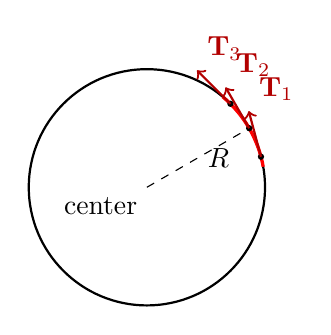
\begin{tikzpicture}[scale=1]
    \def\R{1.5}
    % draw circle and radius
    \draw[thick] (0,0) circle (\R);
    \coordinate (P) at (30:\R);
    \draw[dashed] (0,0) -- (P) node[midway, right] {$R$};
    % highlight a short arc on both sides of P to indicate the region used
    % to measure curvature
    \draw[red,very thick] (10:\R) arc (10:50:\R);
    % draw several unit tangent vectors along the highlighted arc
    \foreach \a/\lab in {15/1,30/2,45/3}{%
        \coordinate (Q\lab) at (\a:\R);
        \fill (Q\lab) circle (0.04);
        \draw[->,red!70!black,thick] (Q\lab) -- ++({\a+90}:0.6) node[above right] {$\mathbf{T}_{\lab}$};
    }
    % center label
    \node at (0,0) [below left] {center};
\end{tikzpicture}
\end{center}

First, find the velocity: $\vec{v}(t) = \langle \answer{-R\sin(t)}, \answer{R\cos(t)} \rangle$

The speed is $|\vec{v}(t)| = \answer{R}$

The unit tangent vector is $\mathbf{T}(t) = \langle \answer{-\sin(t)}, \answer{\cos(t)} \rangle$

Now differentiate with respect to $t$: $\frac{d\mathbf{T}}{dt} = \langle \answer{-\cos(t)}, \answer{-\sin(t)} \rangle$

To find $\frac{d\mathbf{T}}{ds}$, we use: $\frac{d\mathbf{T}}{ds} = \frac{d\mathbf{T}}{dt} \cdot \frac{dt}{ds} = \frac{1}{|\vec{v}|} \frac{d\mathbf{T}}{dt}$

Therefore: $\frac{d\mathbf{T}}{ds} = \frac{1}{R}\langle -\cos(t), -\sin(t) \rangle$
The curvature is $\kappa = \left|\frac{d\mathbf{T}}{ds}\right| = \frac{1}{R}\sqrt{\cos^2(t) + \sin^2(t)} = \answer{1/R}$

\begin{feedback}
Notice that the curvature of a circle is constant everywhere on the circle and equals $\frac{1}{R}$. This confirms our intuition: smaller circles bend more sharply (higher curvature).
\end{feedback}
\end{problem}

\subsection*{The Principal Unit Normal Vector}

Normal vectors are very important in vector calculus. We can create normal vectors to curves in much the same way we created the unit tangent vector, we find the second derivative of the curve with respect to arc length and make it a unit vector (using curvature).

\begin{definition}
The \textbf{Principal Unit Normal Vector} $\mathbf{N}$ is defined as:
\[\mathbf{N} = \frac{1}{\kappa}\frac{d\mathbf{T}}{ds}\]
This vector points in the direction that the curve is bending.
\end{definition}

\begin{problem}
For the circle example above, find the principal unit normal vector at a general point.

% TikZ: circle with eight unit normal vectors placed around it
\begin{center}
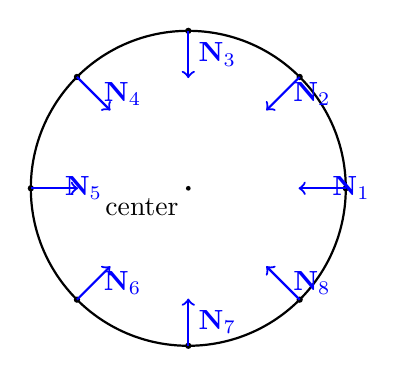
\begin{tikzpicture}[scale=1]
    \def\R{2}
    % circle
    \draw[thick] (0,0) circle (\R);
    % draw 8 points and unit normal vectors (pointing inward)
    \foreach \a/\i in {0/1,45/2,90/3,135/4,180/5,225/6,270/7,315/8}{%
        \coordinate (P\i) at (\a:\R);
        \fill (P\i) circle (0.04);
        % unit normal points radially inward; draw arrow of fixed length
        \draw[->,blue,thick] (P\i) -- ++(\a+180:0.6) node[midway, right] {$\mathbf{N}_{\i}$};
    }
    % center marker
    \fill (0,0) circle (0.03);
    \node at (0,0) [below left] {center};
\end{tikzpicture}
\end{center}

We have $\frac{d\mathbf{T}}{ds} = \frac{1}{R}\langle -\cos(t), -\sin(t) \rangle$ and $\kappa = \frac{1}{R}$

The normal vector is (enter functions of t): $\mathbf{N} = \frac{1}{\kappa}\frac{d\mathbf{T}}{ds} = \langle \answer{-\cos(t)}, \answer{-\sin(t)} \rangle$

\begin{feedback}
Notice that $\mathbf{N}$ points toward the center of the circle! This makes geometric sense: the circle is bending toward its center at every point.

You can verify that $\mathbf{T} \cdot \mathbf{N} = (-\sin(t))(-\cos(t)) + (\cos(t))(-\sin(t)) = 0$, confirming they are perpendicular.
\end{feedback}
\end{problem}

\section*{Computing Curvature and Normal Vectors}

Even though arc-length computations are time-independent, they still need to be computed with respect to time. This excalates the calculational complexity quickly because of factors like the chain rule or other derivative rules.

Below are some formulas that can efficiently compute curvature and normal vectors, for more detail on these formluas check the textbook:

\begin{remark}
Curvature:

\begin{enumerate}
    \item $\kappa = \frac{1}{|\vec{v}|}\left|\frac{d\mathbf{T}}{dt}\right|$ where $\vec{v} = \frac{d\mathbf{r}}{dt}$ and $\mathbf{T} = \frac{\vec{v}}{|\vec{v}|}$
    \item $\kappa = \frac{|\vec{v} \times \vec{a}|}{|\vec{v}|^3}$ where $\vec{a} = \frac{d\vec{v}}{dt}$
\end{enumerate}

Principal Unit Normal Vector:

\begin{enumerate}
    \item $\mathbf{N} = \frac{1}{\kappa}\frac{d\mathbf{T}}{ds} = \frac{1}{\kappa |\vec{v}|}\frac{d\mathbf{T}}{dt}$
    \item $\mathbf{N} = \frac{\frac{d\mathbf{T}}{dt}}{\left|\frac{d\mathbf{T}}{dt}\right|}$
\end{enumerate}
\end{remark}

% \section*{Task Three: The TNB Frame}

% \subsection*{Building a Moving Coordinate System}

% For curves in 3D space, we can construct a complete coordinate system that moves along with a particle. This is called the \textbf{TNB frame} or \textbf{Frenet frame}.

% \begin{definition}
% The TNB frame consists of three mutually perpendicular unit vectors:
% \begin{itemize}
%     \item $\mathbf{T}$: Unit tangent vector (direction of motion)
%     \item $\mathbf{N}$: Principal unit normal vector (direction of bending)
%     \item $\mathbf{B}$: Binormal vector, defined as $\mathbf{B} = \mathbf{T} \times \mathbf{N}$
% \end{itemize}
% \end{definition}

% \begin{problem}
% What properties should the binormal vector $\mathbf{B}$ have?

% \begin{selectAll}
%     \choice[correct]{$\mathbf{B}$ is perpendicular to $\mathbf{T}$}
%     \choice[correct]{$\mathbf{B}$ is perpendicular to $\mathbf{N}$}
%     \choice[correct]{$\mathbf{B}$ is a unit vector}
%     \choice{$\mathbf{B}$ points in the direction of motion}
% \end{selectAll}

% \begin{feedback}
% Since $\mathbf{B} = \mathbf{T} \times \mathbf{N}$ and both $\mathbf{T}$ and $\mathbf{N}$ are unit vectors that are perpendicular to each other, $\mathbf{B}$ is automatically perpendicular to both and has length 1.

% The binormal vector points in the direction perpendicular to the plane containing $\mathbf{T}$ and $\mathbf{N}$ (called the osculating plane).
% \end{feedback}
% \end{problem}

% \begin{problem}
% For the helix $\mathbf{r}(t) = \langle \cos(t), \sin(t), t \rangle$ at $t = 0$:

% First, $\vec{v}(0) = \langle \answer{-\sin(0)}, \answer{\cos(0)}, \answer{1} \rangle = \langle 0, 1, 1 \rangle$

% The speed is $|\vec{v}(0)| = \answer{\sqrt{2}}$

% So $\mathbf{T}(0) = \langle \answer{0}, \answer{1/\sqrt{2}}, \answer{1/\sqrt{2}} \rangle$

% (For this problem, you can assume that $\mathbf{N}(0) = \langle -1, 0, 0 \rangle$)

% The binormal vector is:
% \[\mathbf{B}(0) = \mathbf{T}(0) \times \mathbf{N}(0) = \begin{vmatrix} \mathbf{i} & \mathbf{j} & \mathbf{k} \\ 0 & 1/\sqrt{2} & 1/\sqrt{2} \\ -1 & 0 & 0 \end{vmatrix}\]

% $\mathbf{B}(0) = \langle \answer{0}, \answer{1/\sqrt{2}}, \answer{-1/\sqrt{2}} \rangle$

% \begin{feedback}
% The TNB frame gives us a coordinate system that travels along with the particle. At each point, $\mathbf{T}$ points forward, $\mathbf{N}$ points toward where the curve is bending, and $\mathbf{B}$ points ``out of the plane'' of the curve.
% \end{feedback}
% \end{problem}

% \section*{Task Four: Acceleration in the TNB Frame}

% \subsection*{Decomposing Acceleration}

% One of the most powerful applications of the TNB frame is understanding acceleration. We can decompose the acceleration vector into components along $\mathbf{T}$ and $\mathbf{N}$.

% \begin{definition}
% The acceleration vector can be written as:
% \[\mathbf{a} = a_T \mathbf{T} + a_N \mathbf{N}\]

% where:
% \begin{itemize}
%     \item $a_T = \frac{d|\vec{v}|}{dt}$ is the \textbf{tangential component} (change in speed)
%     \item $a_N = \kappa |\vec{v}|^2$ is the \textbf{normal component} (change in direction)
% \end{itemize}
% \end{definition}

% \begin{problem}
% Let's build intuition about these components. When a car goes around a curve at constant speed:

% What is the tangential component of acceleration?
% \begin{multipleChoice}
%     \choice[correct]{Zero (speed isn't changing)}
%     \choice{Positive (car is speeding up)}
%     \choice{Negative (car is slowing down)}
% \end{multipleChoice}

% What about the normal component?
% \begin{multipleChoice}
%     \choice{Zero (no acceleration)}
%     \choice[correct]{Non-zero (direction is changing)}
%     \choice{Undefined}
% \end{multipleChoice}

% \begin{feedback}
% When speed is constant, $a_T = 0$. But if the car is turning (changing direction), there must be acceleration toward the center of the turn. This is the normal component $a_N$, which depends on both the curvature of the path and the speed.

% This is why you feel pushed to the side when a car turns—that's the normal acceleration!
% \end{feedback}
% \end{problem}

% \begin{problem}
% Consider a particle moving along $\mathbf{r}(t) = \langle t, t^2 \rangle$ at $t = 1$.

% Velocity: $\vec{v}(t) = \langle \answer{1}, \answer{2t} \rangle$, so $\vec{v}(1) = \langle 1, 2 \rangle$

% Speed: $|\vec{v}(1)| = \answer{\sqrt{5}}$

% Acceleration: $\mathbf{a}(t) = \langle \answer{0}, \answer{2} \rangle$, so $\mathbf{a}(1) = \langle 0, 2 \rangle$

% To find $a_T$, we compute $\frac{d|\vec{v}|}{dt}$:
% \[|\vec{v}(t)| = \sqrt{1 + 4t^2}\]
% \[\frac{d|\vec{v}|}{dt} = \frac{4t}{\sqrt{1+4t^2}}\]

% At $t=1$: $a_T = \frac{4}{\sqrt{5}} = \answer[tolerance=0.01]{1.789}$

% To find $a_N$, we can use: $|\mathbf{a}|^2 = a_T^2 + a_N^2$

% $|\mathbf{a}(1)| = \answer{2}$

% $a_N^2 = 4 - \frac{16}{5} = \frac{4}{5}$

% $a_N = \answer[tolerance=0.01]{0.894}$

% \begin{feedback}
% The tangential component tells us the particle is speeding up (positive $a_T$). The normal component tells us the path is curving. Together, these give us complete information about the acceleration.
% \end{feedback}
% \end{problem}

% \section*{Summary and Key Takeaways}

% \begin{problem}
% Let's review the key concepts. Match each quantity to its meaning:

% The curvature $\kappa$ measures:
% \begin{multipleChoice}
%     \choice{How fast a particle is moving}
%     \choice[correct]{How sharply a curve is bending}
%     \choice{The direction of motion}
%     \choice{The speed of the particle}
% \end{multipleChoice}

% The unit tangent vector $\mathbf{T}$ points:
% \begin{multipleChoice}
%     \choice{Toward the center of curvature}
%     \choice[correct]{In the direction of motion}
%     \choice{Perpendicular to the curve}
%     \choice{Opposite to the velocity}
% \end{multipleChoice}

% The principal unit normal $\mathbf{N}$ points:
% \begin{multipleChoice}
%     \choice{In the direction of motion}
%     \choice[correct]{In the direction the curve is bending}
%     \choice{Perpendicular to the osculating plane}
%     \choice{Opposite to acceleration}
% \end{multipleChoice}

% The tangential acceleration component $a_T$ measures:
% \begin{multipleChoice}
%     \choice{Change in direction}
%     \choice[correct]{Change in speed}
%     \choice{Curvature of the path}
%     \choice{Distance traveled}
% \end{multipleChoice}
% \end{problem}

% \begin{problem}
% True or False: Select all TRUE statements.

% \begin{selectAll}
%     \choice[correct]{A straight line has zero curvature}
%     \choice[correct]{The TNB frame provides a moving coordinate system along a curve}
%     \choice{The binormal vector is always constant along a curve}
%     \choice[correct]{Normal acceleration exists whenever direction is changing}
%     \choice[correct]{At constant speed, tangential acceleration is zero}
%     \choice{Curvature depends on how fast a particle moves along the curve}
% \end{selectAll}

% \begin{feedback}
% Great work! Remember that curvature is a geometric property of the curve itself, independent of how fast something moves along it. The TNB frame captures the geometry of spatial curves, extending the ideas of derivatives and concavity from single-variable calculus to three dimensions.
% \end{feedback}
% \end{problem}



\end{document}